% draft.tex

\documentclass{article} % For LaTeX2e
\usepackage{nips13submit_e,times}
% \usepackage{hyperref} % commented out due to errant warning... something to do with using math in a section
\usepackage{url}
\usepackage{amsmath}
\usepackage{graphicx}
%\documentstyle[nips13submit_09,times,art10]{article} % For LaTeX 2.09

\newcommand{\E}{\mathrm{E}}

\newcommand{\Var}{\mathrm{Var}}

\newcommand{\Cov}{\mathrm{Cov}}


\title{Predicting the Outcome of College Basketball Tournament Using a Least-Squares Network Model}


\author{
% David S.~Hippocampus\thanks{ Use footnote for providing further information
% about author (webpage, alternative address)---\emph{not} for acknowledging
% funding agencies.} \\
% Department of Computer Science\\
% Cranberry-Lemon University\\
% Pittsburgh, PA 15213 \\
% \texttt{hippo@cs.cranberry-lemon.edu} \\
Yosuke Sugishita\\
CS490\\
\texttt{yosuke.sugi@gmail.com}
\And
Henry Li\\
CS490 \\
\texttt{henry.s.leigh@gmail.com} \\
}

% The \author macro works with any number of authors. There are two commands
% used to separate the names and addresses of multiple authors: \And and \AND.
%
% Using \And between authors leaves it to \LaTeX{} to determine where to break
% the lines. Using \AND forces a linebreak at that point. So, if \LaTeX{}
% puts 3 of 4 authors names on the first line, and the last on the second
% line, try using \AND instead of \And before the third author name.

\newcommand{\fix}{\marginpar{FIX}}
\newcommand{\new}{\marginpar{NEW}}

\nipsfinalcopy 	% Uncomment for camera-ready version
				% Need this to see authors for whatever reason

\begin{document}


\maketitle

\begin{abstract}
Ranking sports teams and predicting their games' outcome is often said to be a difficult problem.  In this paper, we propose a simple least squares network model to rank teams in the American college basketball league, and attempt to predict the final tournament's outcome.  By training on the past 18 tournaments, we find that our model accurately predicts the outcome of a game in the final tournament with 70$(\pm4)$\% accuracy.  We first train the model using a basic least square model, and proceed to train the same model using $\ell_2$-regularization, which stabilizes our predicted outcome of a new game.
\end{abstract}

\section{Introduction}
\subsection{Background Information (Description of Data)}
The biggest tournament in the American college basketball league is NCAA Basketball, which is commonly referred to as ``March Madness''.  It is a single-elimination tournament played by 67 teams, meaning there are 66 games' outcome to predict.  Roughly 3000 games are played amongst more than 300 teams in our data set every year during the regular season, which we are going to use for tranining our model.
\subsection{Objective (Predictive Accuracy)}
Our objective is to predict this year's (the 2014 season) tournament's outcome and we aim to maximize the simple predictive accuracy of win/lose.  Therefore, we are going to use past years' tournament results as our test data set.  The tested accuracy of a model is defined as follows: 
\begin{equation}
    \mbox{tested accuracy} = \frac{\mbox{number of correct predictions}}{\mbox{number of all predictions}}
\end{equation}

\section{Model}
\subsection{Model Construction}
We define differences 
\[
\hat{d}_{ij} = \hat{x}_i - \hat{x}_j
\]
where $\hat{x}_k$ is the `potential' for a team $k$. These differences represent the difference in final score between a pair of teams $i,j$ given that they have played a game against each other. Now if $\hat{d}_{ij} > 0$, we know that team $x_i$ had won, since $\hat{x}_i > \hat{x}_j$. Using this encoding, we can formalize an equation with which we can form predictions. With $\hat{d}$ as an estimator of the resulting score, we can minimize the square differences 
\[
\min_{x_i}\sum_{\texttt{all games}}\left(d_{ij}-\hat{d}_{ij} \right)^2
\]
\subsubsection{Training the Model}
In training the model, we take the data comprising of games played by 300 teams over the course of 18 seasons. Additionally, in each tournament, there were anywhere from 63 to 67 games. We encode this data as an incidence matrix 
\[\mathbf{A} = \begin{bmatrix}
  a_{t_1g_1} & a_{t_2g_1} & \cdots & a_{t_ng_1}\\
  a_{t_1g_2} & a_{t_2g_2} & \cdots & a_{t_ng_2}\\
  \vdots & \vdots & \ddots & \vdots\\
  a_{t_1g_n} & a_{t_2g_n} & \cdots & a_{t_ng_n}
\end{bmatrix} \]
where each column represents one team in a given season and row represents a game played; since a game can only be played between two teams, each row contains exactly 2 non-zero elements. Further, for the two teams involved in some game $g_k$, we apply the convention that the `first' team $t_i$, that is the team whose column appears before the `second' tema $t_j$ such that $i<j$, obtains the value $a_{t_ig_k} = -1$ for the element while $a_{t_jg_k} = -1$. Not surprisingly this forms the machinery needed to perform many calculations of $\hat{d}$ and thus to assign potentials to each team.

But to do this, we need to solve a system involving the actual scores for games within some tournament within the data. Let $\mathbf{s}$ be the vector of differences between all final scores of each game in the tournament. Then to determine the potentials for each team, is a matter of solving the system 
\[\mathbf{A}\mathbf{x} = \mathbf{s} \]
As a simple example with 4 teams and 3 games (we assume that teams 1 and 3 are carried forth onto the second round), we have:
\[
\begin{bmatrix}
  1&-1&0&0\\
  0&0&1&-1\\
  1&0&-1&0
\end{bmatrix}\begin{bmatrix}
  x_1\\x_2\\x_3\\x_4
\end{bmatrix} = \begin{bmatrix}
  32\\20\\-2
\end{bmatrix}
\]
In this case, solving for $\mathbf{x}$ would return the potentials for each of the 4 teams.
\subsubsection{Testing the Prediction Accuracy}
\subsection{Confidence Interval Analysis}
$\sim$
\subsection{Use of $\ell_2$-Regularization}\label{sec:l2}

\section{Results}
\subsection{Predictive Accuracy}
We achieved roughly $70(\pm4)\%$ accuracy for predicting the past 18 tournaments' outcome (for win/lose prediction).  This is an out-of-sample result as we trained our model on the same seaosn's regular game results, which preceed the tournament.
\subsection{Regularization (Irregular Behaviour in the Results)}
We noticed that differences between our potential estimates are sometimes unusually high or low (for instance, in the order of $10^9$).  One can see this effect easily from the average standard deviation of potential estimates for each year (Table ~ \ref{table:std}).

\begin{table}
\begin{center}
  \begin{tabular}{ | l | c | r | }
    \hline
    Regularization parameter & Average standard deviation of potential estimates \\ \hline
    0 (no regularization) & 1.351e+15 \\ \hline
    $10^{-12}$ & 5.758\\ \hline
    $10^{-9}$ & 5.758\\ \hline
    $0.001$ & 5.757\\
    \hline
  \end{tabular}
  \caption{Average standard deviation of potential estimates}
  \label{table:std}
\end{center}
\end{table}

As the potential differences are used as the predicted score difference of a game, this is clearly an irregular result.  Also, as we examined the plot of predicted score differences against actual scores, we realized that the predictions can be unstable particularly when the actual score differences are small (when the games are ``close''). 

\begin{figure}[ht!]
    \centering
    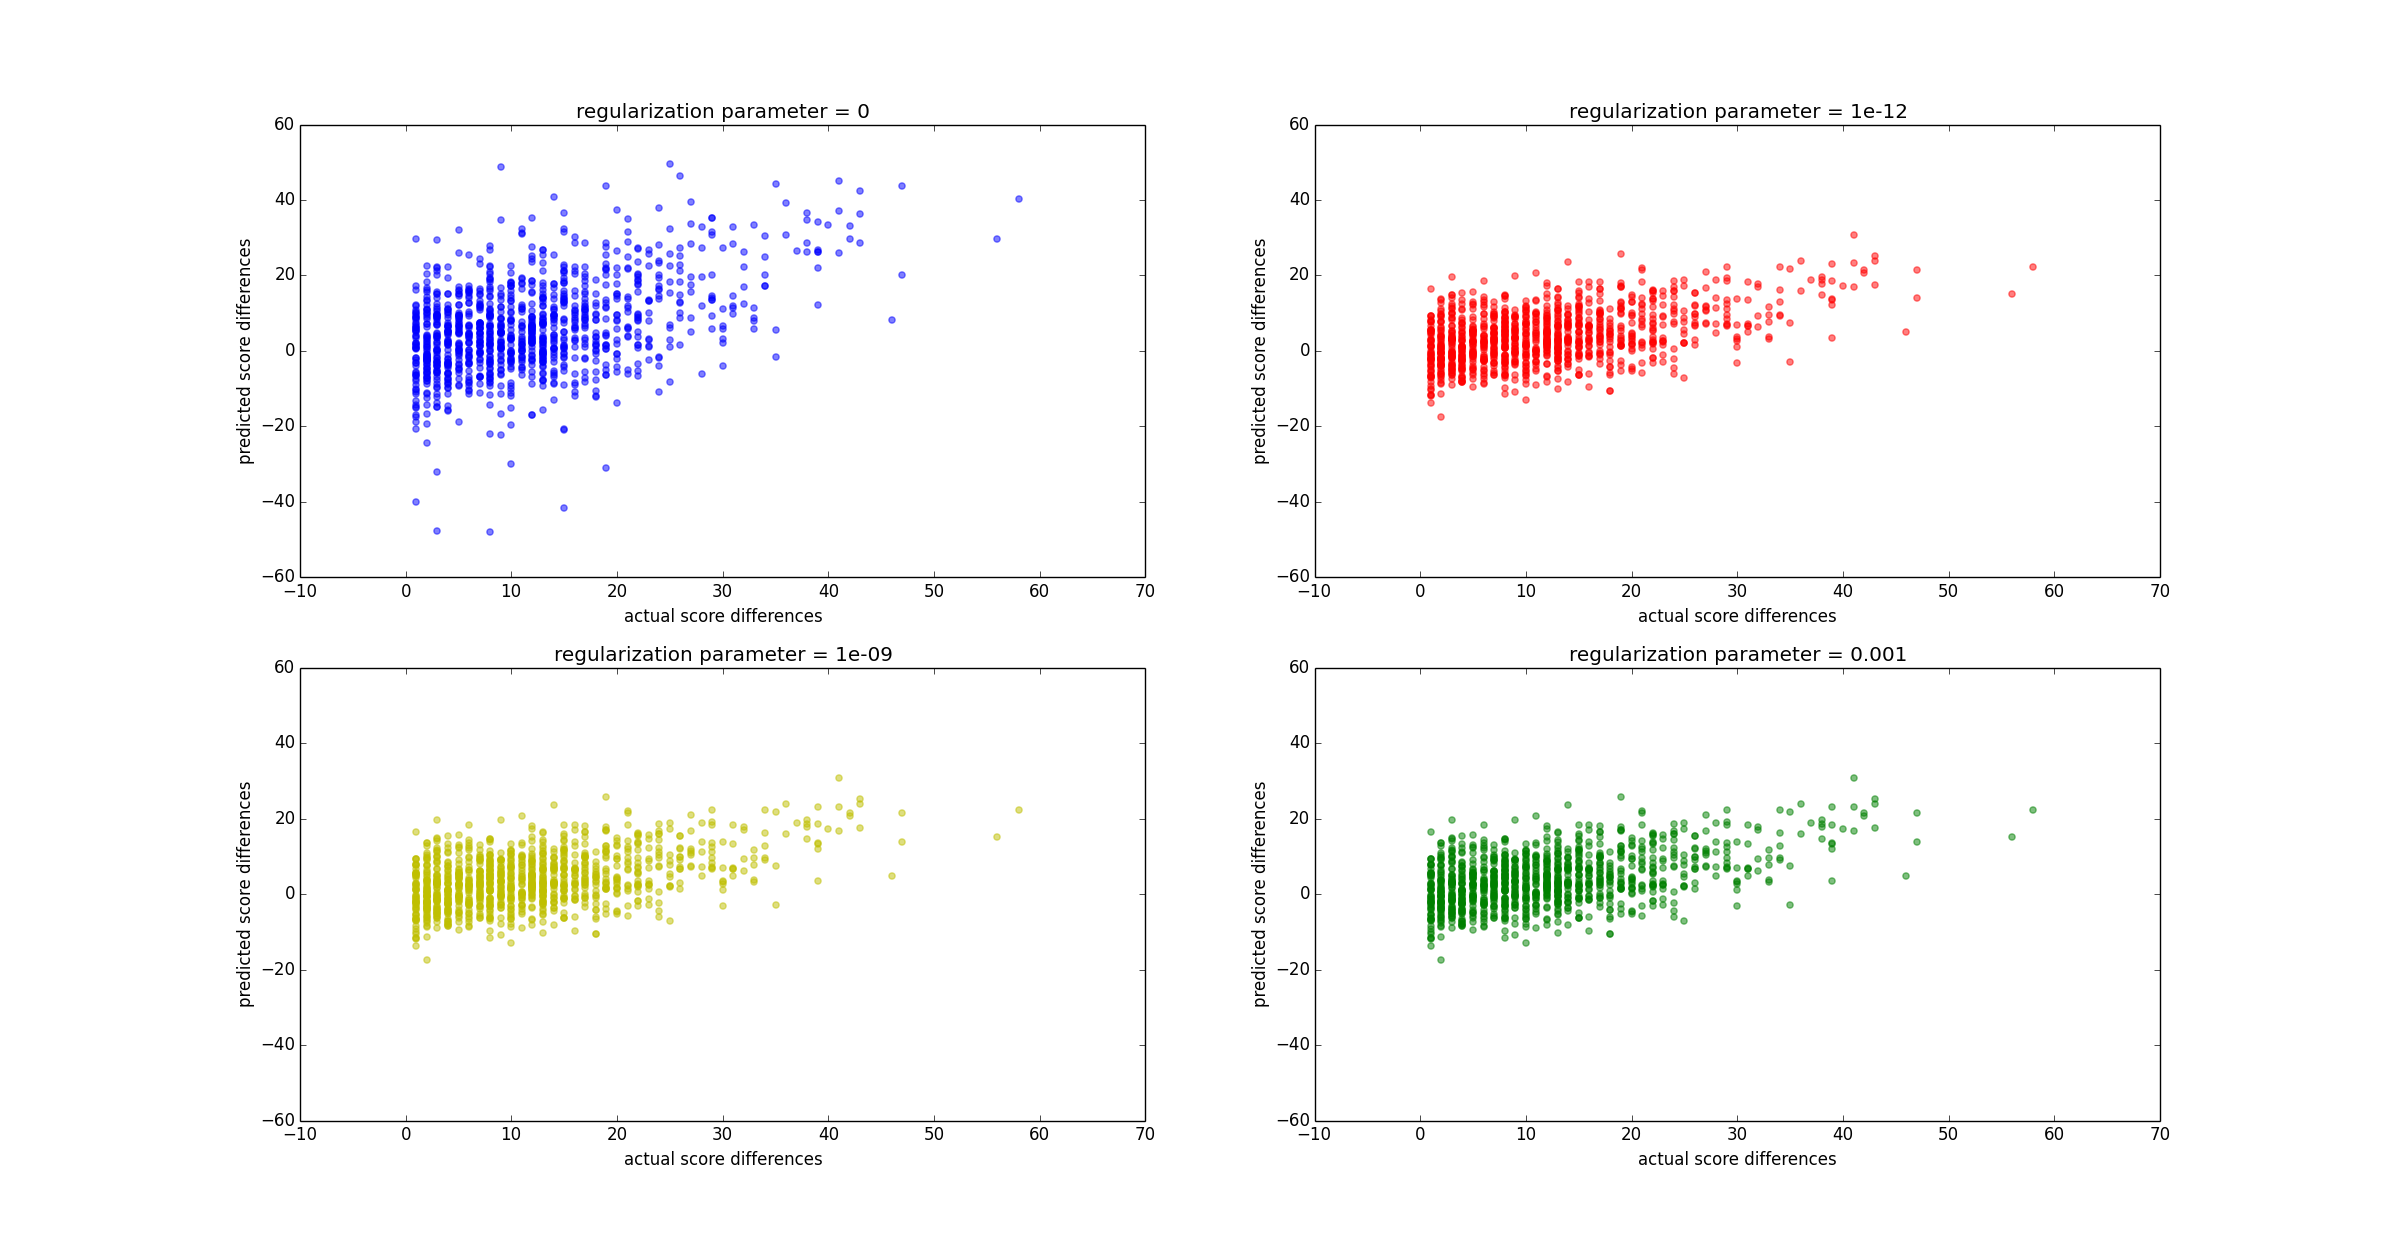
\includegraphics[width=140mm]{actual_vs_predict.png}
    \caption{Predicted score differences against actual score differences}
    \label{actual_vs_predict}
\end{figure}

To prevent these unusual behaviors and also to stabilize the predictions, we utilized $\ell_2$-regularization.  The model is described in Section~\ref{sec:l2}: $\ell_2$-Regularization.  As expected, this model yielded more stable predictions as shown in Figure~\ref{actual_vs_predict}.  This was also clear when we compared the correlation coefficients between actual score differences and predicted score differences (it improved from 0.456 to 0.468.  However, it did not change the predictive accuracy significantly.

Interestingly, ranging the regularization parameter from $10^{-9}$ to $0.001$ hardly changed the results as can be seen from Figure~\ref{actual_vs_predict}.


\section{Conclusion}
\subsection{Summary}
\subsection{Further Considerations}



% 1. Introduction
% 1.1. Background information (description of data)
% 1.2. Objective (predictive accuracy)

% 2. Model
% 2.1. Model construction
% 2.1.1. Traning the model
% 2.1.2. Testing the accuracy
% 2.2. Confidence interval
% 2.3. L2-regularization

% 3. Results
% 3.1. Predictive accuracy
% 3.2. Regularization (irregular behavior in the results)

% 4. Conclusion
% 4.1. Summary
% 4.2. Further considerations



\end{document}
